\documentclass[a4paper, 12pt]{article}

\usepackage[italian]{babel}
\usepackage{graphicx}
\usepackage{float}

\linespread{1.3}



\title{Sintesi di Composti d'interesse Medico per il Trattamento del Morbo d'Alzheimer}
\author{
	Relatore: Annamaria DeAgostino
	\and
	Candidato: Lorenzo Castellino
}
\date{Anno Accademico 2018-2019}

\begin{document}
\pagenumbering{gobble}
\maketitle
\setcounter{page}{0}
\newpage
\tableofcontents
\newpage
\pagenumbering{arabic}

\section{Introduzione al Morbo d'Alzheimer}
La malattia di Alzheimer-Perusini, nota più comunemente come morbo d'Alzheimer (AD), è una tra le forme più diffuse al mondo di demenza senile. Dal punto di vista medico la patologia è definita come "disturbo neurocognitivo maggiore o lieve dovuto a malattia di Alzheimer".\cite{american_psychiatric_association_diagnostic_2013}
I sintomi associati sono differenti da individuo ad individuo, in generale nei pazienti riconosciuti si sono osservate:
\begin{enumerate}
	\item Perdita di memoria a breve termine.
	\item Difficoltà a concentrarsi, organizzarsi e di pianificazione.
	\item Difficoltà a seguire e/o formulare discorsi di senso compiuto.
	\item Difficoltà a giudicare distanze e spazi.
	\item Perdita di orientamento spaziale e temporale.
	\item Cambi repentini dell'umore.
	\item Allucinazioni visive.
\end{enumerate}
La demenza è una patologia di tipo progressivo, ovvero si ha un peggiormento dei sintomi col passare del tempo. La velocità di tale processo varia da persona a persona, tendenzialmente l'aspettativa media di vita successiva alla diagnosi della condizione va dai 3 ai 10 anni. \cite{todd_survival_2013}

\subsection{L'Importanza della Ricerca}
L'incidenza dell'AD è in aumento tanto da individuare nella ricerca di una cura come una delle sfide per il nuovo millenio: stando al World Alzheimer Report del 2018, stilato dall'Alzheimer's Disease International ovvero l'associazione internazionale per la lotta all'Alzheimer in stretta collaborazione con la World Health Organization, si stima che nel mondo circa 50 milioni di persone siano affette da demenza. Ciò si traduce in una spesa annua per il trattamento dei malati che rasenta il miliardo di dollari.

Con l'aumento dell'aspettativa media di vita si prevede che nel 2050 il numero di casi sarà il triplo di quello odierno e si prospetta una spesa doppia rispetto a quella attuale.\cite{noauthor_world_2018}

Stando a queste previsioni 1'individuo su 85 nel 2050 sarà affetto da demenza.

L'individuazione delle cause che portano al presentarsi dell'AD è uno dei punti salienti della ricerca in campo medico e biochimico, sono state portate avanti molte ipotesi a riguardo. Al momento una delle tesi più avvalorate e studiate è quella della formazione di aggregati proteici nel liquido cerebrospinale.

\subsection{L'Ipotesi della Cascata Amiloidica}
Con il termine $\beta$-amiloide (A$\beta$) si indica un aggregato proteico composto da fibrille microscopiche non ramificate, il nome è dovuto al fatto che al momento della scoperta, viste le sue proprietà si pensò in ad una similitudine con le molecole d'amido benchè dal punto di vista della composizione chimica non ci siano particolari somiglianze.\cite{lennarz_encyclopedia_2004}

L'origine di queste strutture è legata all'azione congiunta di tre enizmi ($\alpha$-secretasi,$\beta$-secretasi e $\gamma$-secretasi) su di un substrato proteico noto come APP (Amyloid Precursor Protein). L'APP è una proteina trans-membrana di modeste dimensioni (circa 700 residui), viene trasportata lungo l'assone delle cellule neuronali e si accumula nei siti presinaptici. Il suo rilascio è regolato dall'attività elettrica cerebrale, si suppone infatti che abbia un ruolo fondamentale nella regolazione dell'eccitabilità neuronale.\cite{mattson_cellular_1997}
La porzione che interessa la formazione di A$\beta$ è situata nel dominio extracellulare dell'APP. Come si può osservare nella Figura \ref{fig:app} i tre enzimi sopracitati agiscono in punti ben definiti e tra loro differenti della proteina; in particolare si osservi come l'azione dell'$\alpha$-secretasi non porti alla formazione del frammento $\beta$A mentre l'azione dell'enzima $\beta$ in congiunzione all'enzima $\gamma$ generi la particolare sequenza.\cite{goedert_century_2006}

\begin{figure}[H]
	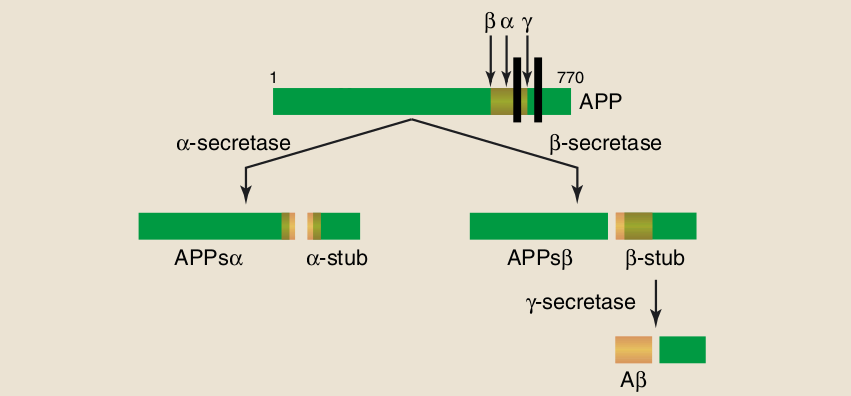
\includegraphics[width=\linewidth]{immagini/APP.png}
	\caption{Azione degli enzimi $\alpha$/$\beta$/$\gamma$-secretasi sul substrato APP.}
	\label{fig:app}
\end{figure}

I frammenti prodotti sono di due varietà che si differenziano per il numero di residui in essi contenuti, ecco quindi che possiamo distinguere i A$\beta$-40 e i A$\beta$-42 rispettivamente formati da 40 e 42 amminoacidi. Il rapporto tra le quantità prodotte delle due forme é di particolare importanza in quanto la $\beta$A-42 tende a formare oligomeri e fibrille più facilmente rispetto all’$\beta$A-40.

La produzione di $\beta$ in piccole quantità é un processo normale; delle funzioni osservate citiamo: \cite{brothers_physiological_2018}

\begin{enumerate}
	\item Funzione antibatterica, antifunginea e antivirale.
	\item Soppressione tumorale.
	\item Meccanismo di riparazione di falle nella barriera emato-encefalica (azione simile alle piastrine nel sangue).
	\item Regolazione dell'attività sinaptica.
\end{enumerate}

Malgrado i benefici per l'organismo una sovrapproduzione di A$\beta$ o una sproporzione verso la forma contenente 42 residui associata ad uno smalitmento non efficacie sembra essere una causa sufficiente per lo sviluppo precoce del Morbo d’Alzheimer. \cite{irvine_protein_2008}

All'aumento della concentrazione di A$\beta$ nel liquido cerebrospinale è infatti associata la tendenza alla formazione di aggregati proteici più grandi ed insolubili detti comunemente "placche". L'accumulo di queste altera la chimica delle sinapsi, rallentando la trasmissione tra neuroni fino al punto di impedirla, causando così infine la morte della cellula.





\newpage

\bibliographystyle{plain}
\bibliography{biblio.bib}
\end{document}
